\section{GraphRA2 Klassenreferenz}
\label{classGraphRA2}\index{GraphRA2@{GraphRA2}}
Klassendiagramm für GraphRA2::\begin{figure}[H]
\begin{center}
\leavevmode
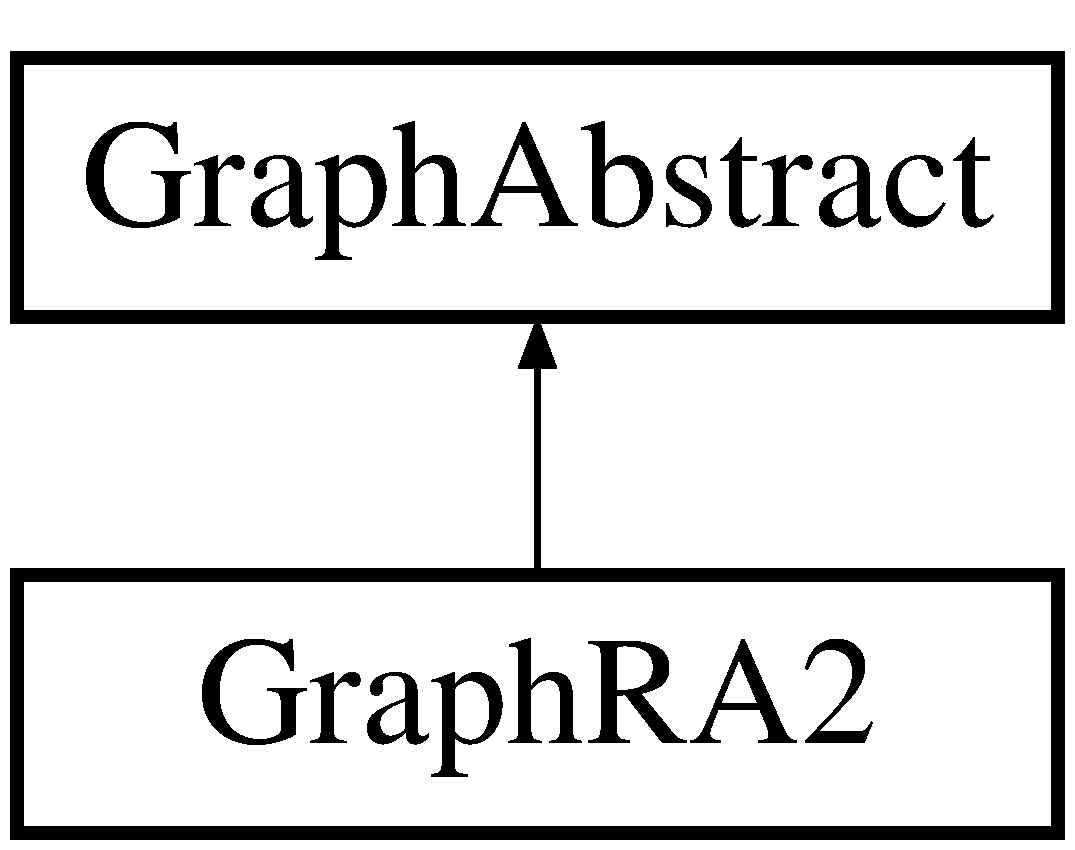
\includegraphics[height=2cm]{classGraphRA2}
\end{center}
\end{figure}
\subsection*{Öffentliche Methoden}
\begin{CompactItemize}
\item 
{\bf GraphRA2} (\$graphId)
\end{CompactItemize}


\subsection{Ausführliche Beschreibung}


Definiert in Zeile 8 der Datei class.GraphRA2.php.

\subsection{Dokumentation der Elementfunktionen}
\index{GraphRA2@{GraphRA2}!GraphRA2@{GraphRA2}}
\index{GraphRA2@{GraphRA2}!GraphRA2@{GraphRA2}}
\subsubsection{\setlength{\rightskip}{0pt plus 5cm}GraphRA2.GraphRA2 (\$ {\em graphId})}\label{classGraphRA2_d0344436a7a552f471eb48f58282402c}




Definiert in Zeile 10 der Datei class.GraphRA2.php.

Die Dokumentation für diese Klasse wurde erzeugt aufgrund der Datei:\begin{CompactItemize}
\item 
{\bf class.GraphRA2.php}\end{CompactItemize}
